\chapter{Introduction}
\label{ch:introduction}

\section{The Earth’s radiation budget}
\label{sec:earth_rad_budget}
The Earth's climate is driven by the energy flow into and out of the system. The incoming solar radiation (yellow fluxes in \figref{fig:earth_energy_budget}) reaches the Earth at the top of the atmosphere (TOA)\index{TOA}, then goes through the atmosphere and arrives at the Earth surface. During this process, approximately two thirds of this shortwave (SW) radiation is absorbed by the Earth surface and atmosphere, and roughly one third of this energy is reflected back to space. The the surface and atmosphere are heated by this incoming solar radiation, and they also re-emit the longwave (LW) radiation (purple fluxes in \figref{fig:earth_energy_budget}) to keep a relatively stable temperature. Globally, the annual mean incoming solar radiation flux is about 340 Wm$^{-2}$, the reflected solar radiation flux is around 100 Wm$^{-2}$ and the outgoing longwave radiation (OLR) is close to 240 Wm$^{-2}$ at the TOA for period 2000--2010 \citep{Stephens2012update}. These three components balance with each other, with a small positive imbalance (about 0.6 Wm$^{-2}$) at the TOA. A more recent estimate from \cite{Wild2015} (see their Fig. 1) indicates that the gloabl mean OLR is about 239 Wm$^{-2}$, and the TOA energy imbalance is about 1 Wm$^{-2}$.
%But due to the accuracy of the observation itself, it is hard to track the causes of these imbalance.

\begin{figure}[ht]
	\centering
	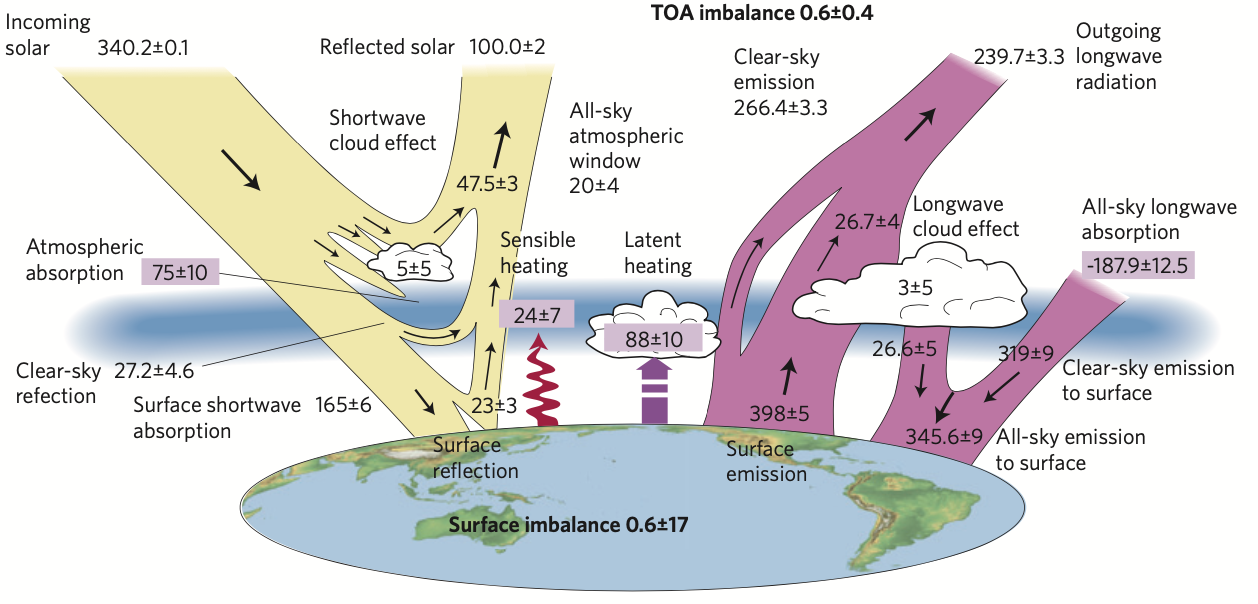
\includegraphics[width=1\linewidth]{{figs/literature_review/earth_enery_budget_Stephens2012}.png}
	\caption[The global annual mean energy budget of Earth for the approximate period 2000–2010 from \cite{Stephens2012update}]{The global annual mean energy budget of Earth for the approximate period 2000–2010. All fluxes are in Wm$^{-2}$. Solar fluxes are in yellow and infrared fluxes in purple. The four flux quantities in purple-shaded boxes represent the principal components of the atmospheric energy balance. Adapted from \cite{Stephens2012update}.}
	\label{fig:earth_energy_budget}
\end{figure}

As shown in \figref{fig:earth_energy_budget}, the energy budget at the Earth's surface is more complicated than at the TOA. When the incoming solar radiation reaches the surface, the majority (about 165 Wm$^{-2}$) of this solar radiation is absorbed by the surface and only a small portion (about 23 Wm$^{-2}$) is reflected back to space. Of course, these are global mean results and it would be different over certain areas such as Arctic where the surface albedo is large. The global annual mean LW radiation emitted from the surface is about 398 Wm$^{-2}$. Much of this is absorbed by the atmosphere (such as the greenhouse gases, aerosols and clouds), and only a small part (about 20 Wm$^{-2}$) can pass through the atmospheric window region (a portion of the infrared spectrum where there is almost no atmospheric absorption) reaching the TOA directly. The atmosphere can re-emit the absorbed LW radiation both upward and downward, and downward part (about 346 Wm$^{-2}$) can reheat the surface. In addition, due to the temperature and moisture difference between the surface and atmosphere, the surface is also cooled by the latent heat flux (about 88 Wm$^{-2}$) and sensible heat flux (about 24 Wm$^{-2}$) through the turbulent movement of atmosphere. In total, the surface energy budget is balanced by the downward/upward SW and LW radiation, the sensible and latent heat fluxes, but it has much larger uncertainty than at the TOA.

\section{Climate feedback}
\label{sec:climate_fbk_intro}

\subsection{Definition}

\begin{figure}[ht]
	\centering
	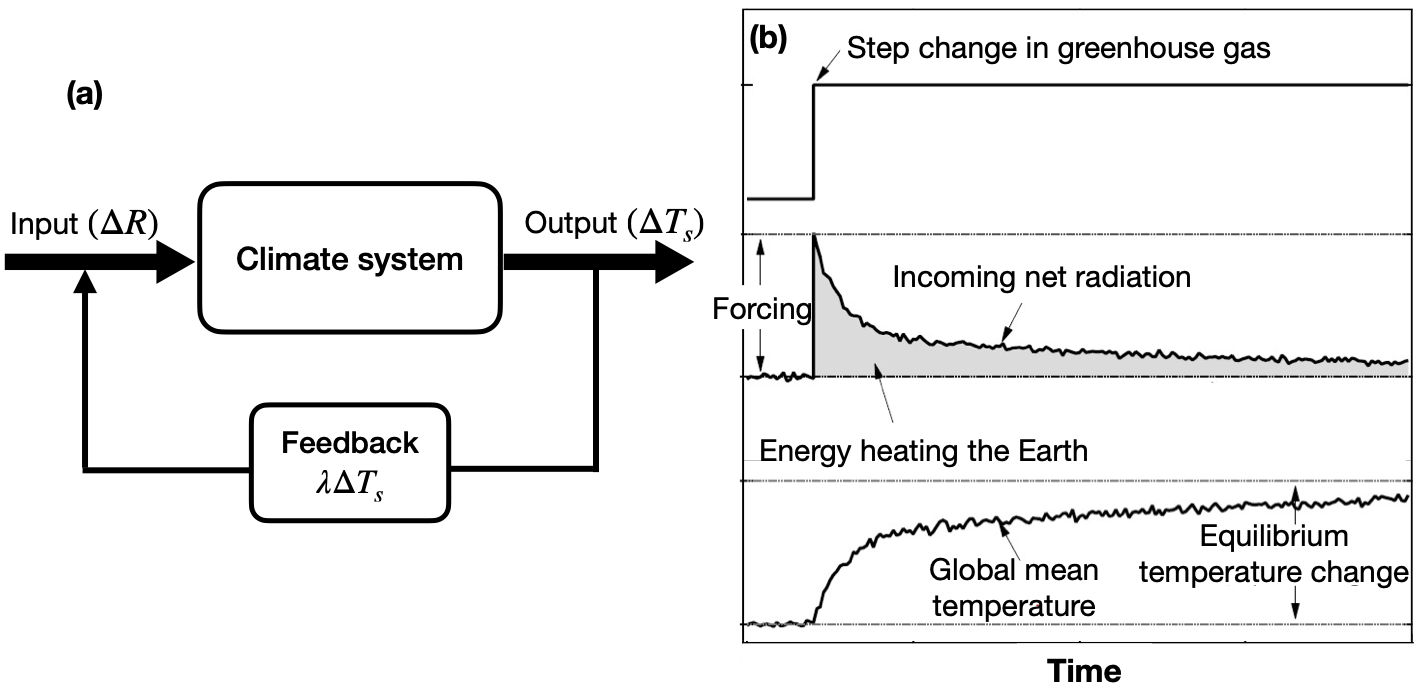
\includegraphics[width=0.95\linewidth]{{figs/literature_review/clim_system_feedback2}.png}
	\caption{(a) Schematic of feedback in climate system. $\Delta R$ is the input disturbance to the climate system, $\Delta T_s$ is the change of surface temperature and $\lambda$ denotes the climate feedback parameter. Modified from Fig. 2 of \cite{Stephens2005cloud}. (b) The illustration of forcing (middle) and global mean temperature (bottom) change with time due to a step change (top) in greenhouse gas, aerosol, etc. Modified from Fig. 1 of \cite{Murphy2009}.}
	\label{fig:schematic_climate_feedback}
\end{figure}

%What is feedback?
 As introduced in \secref{sec:earth_rad_budget}, the energy budget at the TOA is balanced by the incoming solar radiation and the OLR (the imbalance is usually small). Another problem is how to understand the behaviors that the climate system responds to perturbations? In this section, a framework to understand such characters of climate system, including the forcing, feedback, and climate sensitivity will be presented.
 
 In the energy balance model, any disturbance imposed to the system is regarded as the forcing ($\Delta F$), which can be aroused from the perturbation of greenhouse gas concentration (e.g., CO$_2$, CH$_4$), aerosol \citep{Ramanathan2001aerosols}, and change in solar cycle \citep{Frohlich2004solar} or volcanic eruption (\figref{fig:schematic_climate_feedback}). Then climate system will response to this radiative imbalance ($\Delta R$) at the TOA  by changing the surface temperature ($T_s$). As shown in \figref{fig:schematic_climate_feedback}a, the change in surface temperature (i.e. $\Delta T_s$) can in turn impact the radiative balance at the TOA. That is to say the output response is fed back to the system. $\Delta R$ goes to zero during the process when climate system adjusts towards a new equilibrium (\figref{fig:schematic_climate_feedback}b). Using the idea of feedback\index{feedback}, which is taken from the control system and used to understand the system response to different forcings \citep{Stephens2005cloud},
$\Delta R$ can be linked to the change of surface temperature ($\Delta T_s$) as follows:
\begin{equation}
    \Delta R = \Delta F + \lambda \Delta T_s,
    \label{eq:imbalance_forcing_lambda}
\end{equation}
which can be viewed as a Taylor expansion in surface temperature change ($\Delta T_s$), but neglecting the high order terms \citep{Feldl2013a}. The second term, $\lambda \Delta T_s$, on right hand side reflects the radiative flux change that is linearly depend on the surface temperature change, and $\lambda$ is called the \textit{feedback parameter} \citep{Gregory2004}. At the equilibrium state (i.e., $\Delta R=0$), the total climate feedback is expressed as 
\begin{equation}
    \lambda = -\frac{\Delta F}{\Delta T_s}.
\end{equation}
Thus, $\lambda$ is in units of Wm$^{-2}$K$^{-1}$, and is a measure of the TOA radiative flux change per degree of surface air temperature change. 
% Conceptually, \Eqref{eq:imbalance_forcing_lambda} states that the TOA energy imbalance can be expressed as the sum of the radiative forcing and the radiative response of the system to a global surface temperature anomaly.

%\subsection{Climate sensitivity}
Based on the forcing and feedback analysis framework, the equilibrium climate sensitivity (ECS), i.e., the the equilibrium response of global mean surface air temperature to the radiative forcing from a doubling of CO$_2$ ($F_{2\times}$), can be estimated as:
\begin{equation}
    ECS = \Delta T_{s\_2\times}=-\frac{F_{2\times}}{\lambda}.
    \label{eq:ecs}
\end{equation}
ECS is a measure of the climate sensitivity of a general circulation model (GCM) to the forcing, and has a quite large range ($\sim$1.5--4.5K) among the fifth phase of the Coupled Model Intercomparison Project \citep[CMIP5;][]{Taylor2012overview} models \citep[e.g.,][]{Andrews2012forcing,Ceppi2017}, and such a spread (see the first panel in \figref{fig:zelinka_global_mean_fbks}) does not reduce in recent CMIP6 \citep{Eyring2016overview} models  \citep{Zelinka2020causes}. Evidence from historical and paleoclimate records perhaps can help narrow down the uncertainty of ECS \citep{Sherwood2020}, but more work still needed to understand the uncertainty of ECS.
%\cite{Sherwood2020} evaluated the Earth's climate sensitivity based on multiple lines of evidence (feedback process understanding and the historical and paleoclimate records), and find that...

\subsection{Individual feedbacks}
% Introduction of different feedbacks?
In climate system, climate feedbacks are the processes that can either amplify or dampen the effects of climate forcings \citep{Hansen1984}. A feedback that amplifies the initial perturbation is called a ``positive feedback", while a ``negative feedback" reduces the initial perturbation. In general, $\lambda$ can be decomposed into feedbacks from different physical processes, such as temperature (Planck and lapse rate), water vapor, surface albedo, clouds, etc. These climate feedback parameters can be evaluated as follows
\begin{equation}
    \lambda = \frac{\partial R}{\partial T_s} = \sum_x \frac{\partial R}{\partial x}\frac{\partial x}{\partial T_s} + Re, %\text{high-order terms},
    %+ \sum_x\sum_y \frac{\partial^2 R}{\partial x\partial y}\frac{\partial x\partial y}{\partial^2 T_s}+\dots 
    \label{eq:lambda}
\end{equation}
where $x$ represent the climate variable such as temperature, water vapor, surface albedo and cloud properties. $\frac{\partial R}{\partial x}$ can be treated as the feedback parameter due to climate variable $x$. When neglecting the nonlinearities and interactions among different feedbacks, the high-order residual term ($Re$) is usually neglected in analysis. 

The temperature feedback in climate system can be decomposed into Planck and lapse rate feedback \citep{Soden2006}. The Planck feedback assumes that the tropospheric temperature change is vertically uniform and equals to the surface temperature change \citep{Bony2006,Soden2006}, and in other words, there is no vertical temperature change in the troposphere (see second panel in \figref{fig:lapse_rate_fbk_illustration}). The Planck feedback is named due to the Planck's blackbody radiation law, which is the basic and the strongest negative feedback in climate system. According to the Stefan--Boltzmann law, the longwave radiation emitted by the Earth’s surface rises with temperature following $OLR=\epsilon\sigma T_s^4$, where $\epsilon$ is the surface emissivity close to unity and $\sigma=5.67\times 10^{-8}\, \mathrm{W\, m^{-2}\,K^{-4}}$ the Stefan--Boltzmann constant \citep{Pithan2014}. Thus, the Planck feedback can be expressed as $\lambda_P = \frac{\partial R}{\partial T_s}=-4\epsilon\sigma T_s^3=-4\frac{OLR}{T_s}$ (assuming $R$ downward positive). As shown in \figref{fig:earth_energy_budget}, the OLR is closed to 240 Wm$^{-2}$, and the observed global mean surface temperature of Earth is about 288K, thus the estimated Planck feedback is about $\lambda_P=-4\times 240/288\approx -3.3$ Wm$^{-2}$K$^{-1}$, closed to the multi-model mean results in \figref{fig:zelinka_global_mean_fbks}. As the physical law to control the Planck feedback is quite solid, its intermodel spread is the smallest among all the climate feedback parameters in models from the CMIP5 and CMIP6 (see \figref{fig:zelinka_global_mean_fbks}).

\begin{figure}[ht]
	\centering
	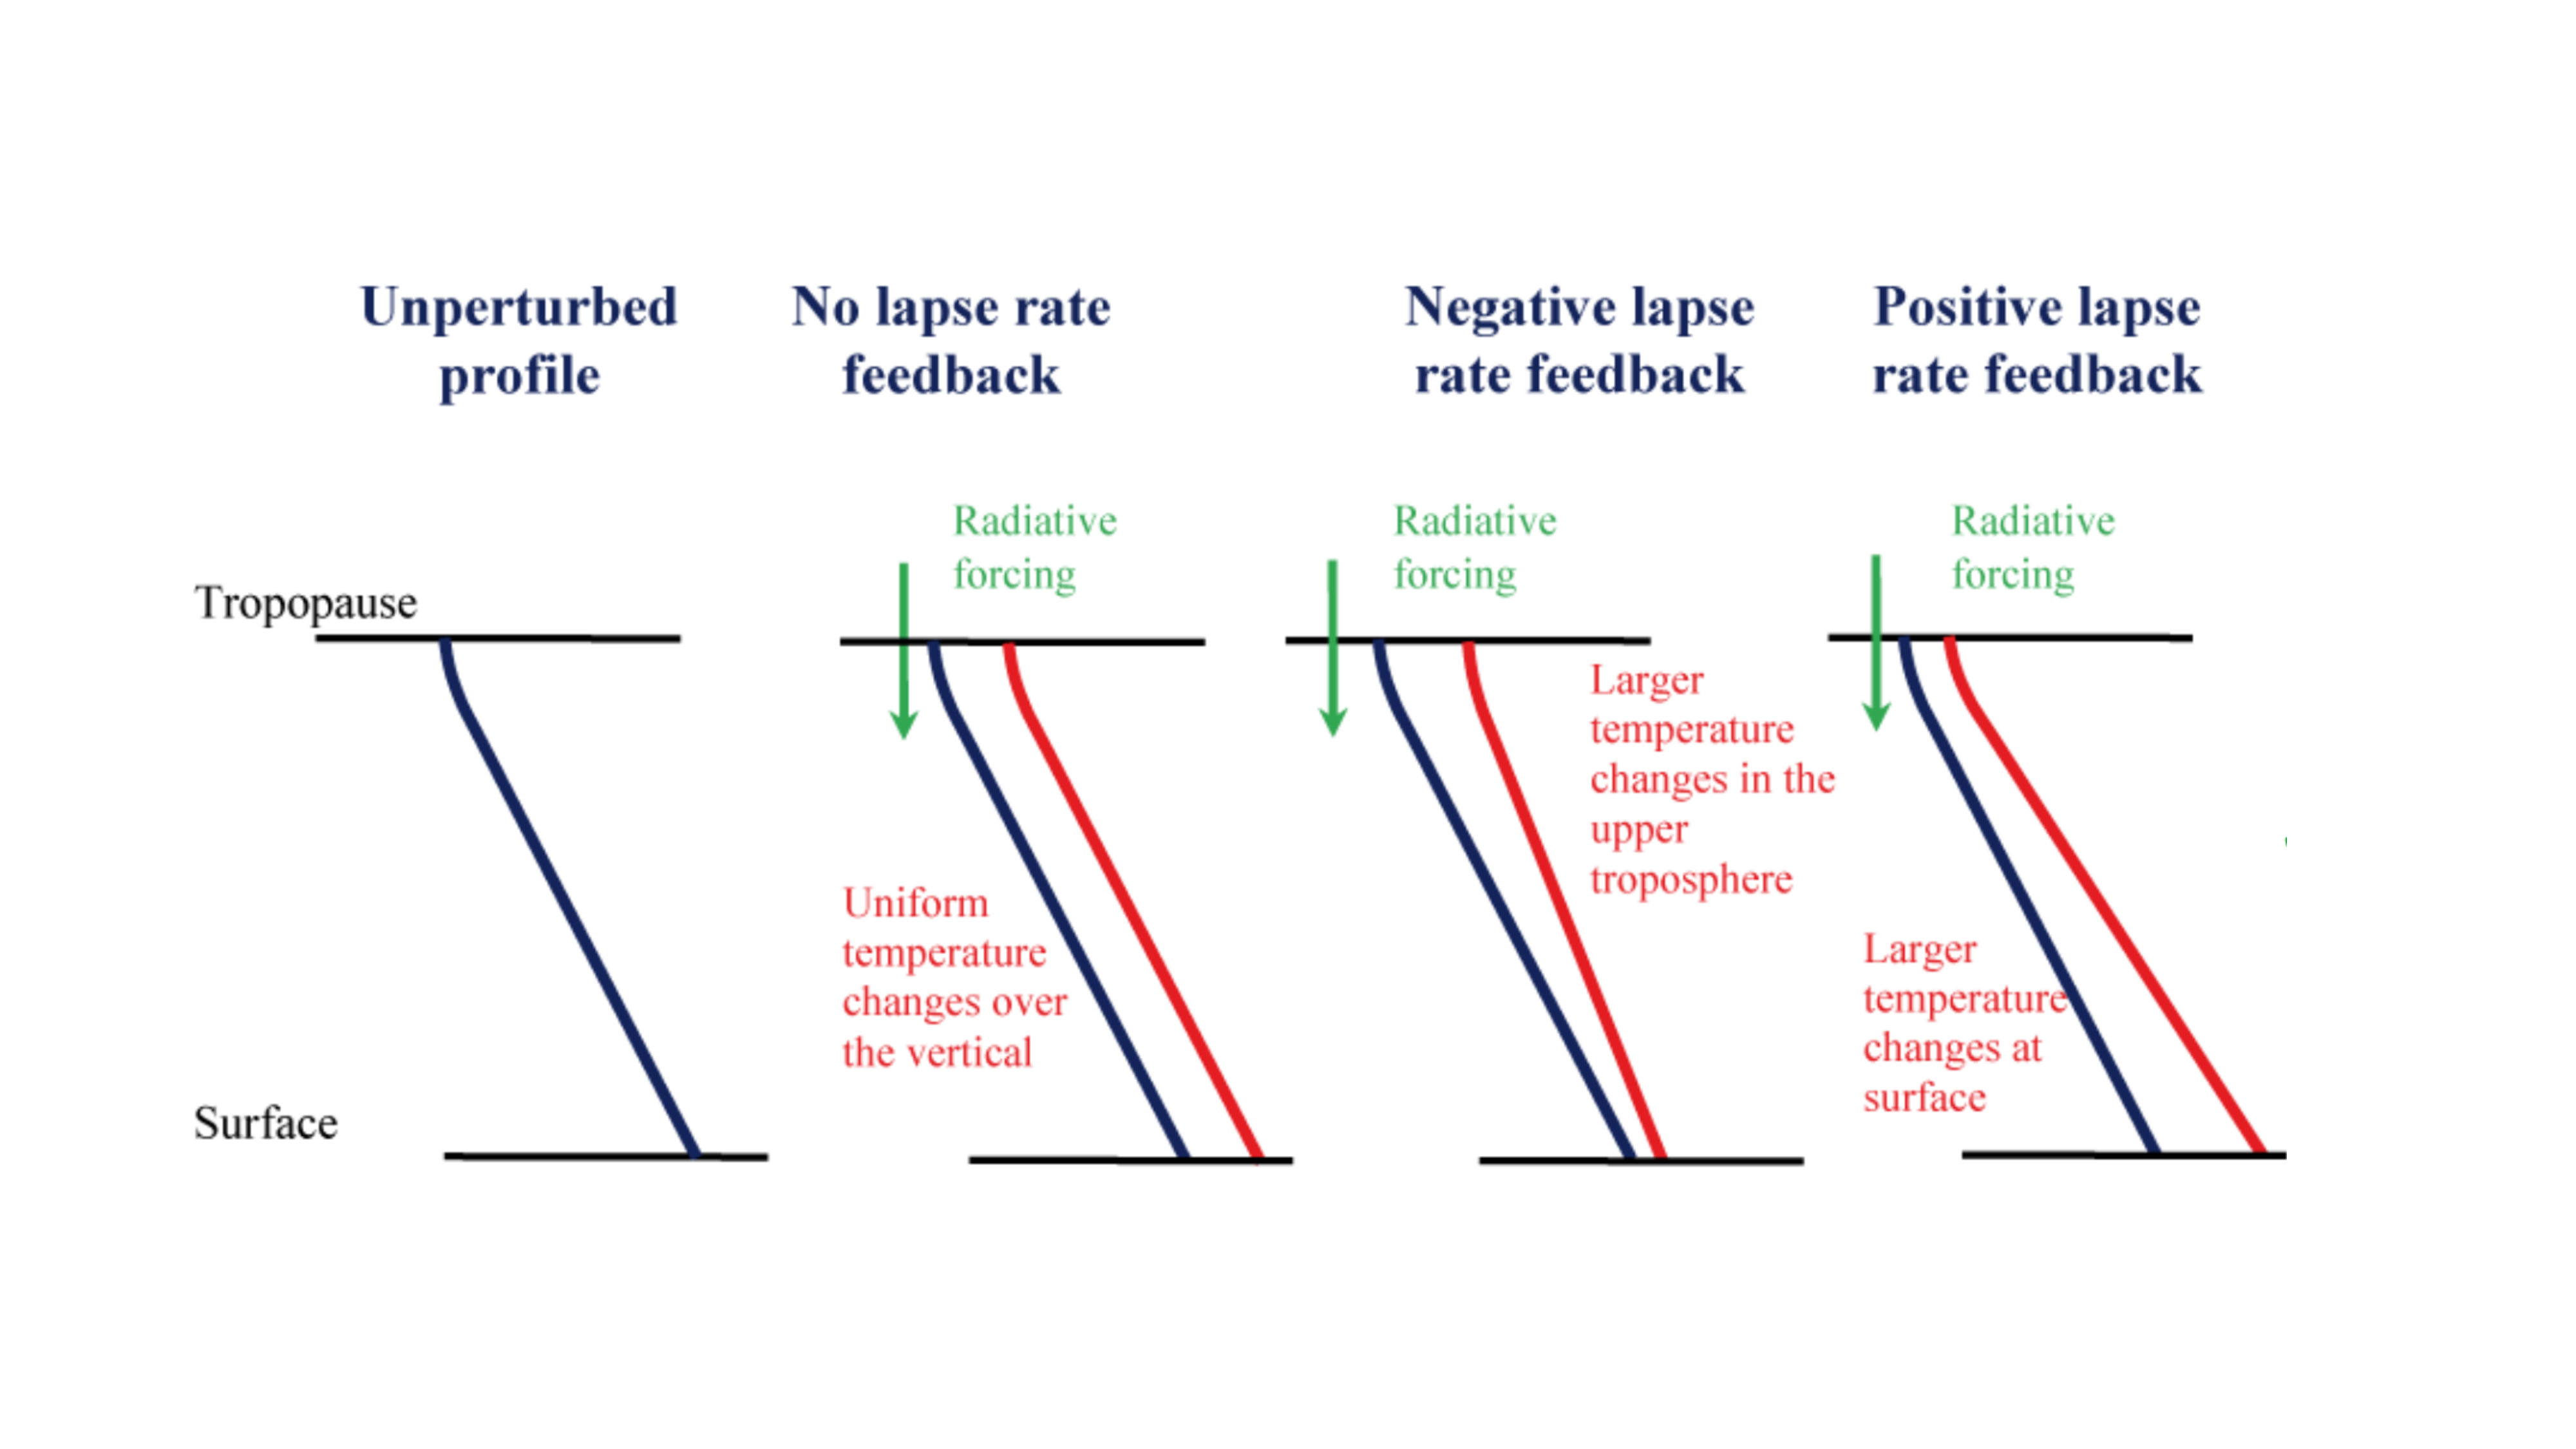
\includegraphics[width=0.95\linewidth]{{figs/literature_review/lapse_rate_fbk}.pdf}
	\caption{Schematic representation of positive and negative lapse-rate feedbacks. The dark blue and red lines are for the unperturbed and perturbed temperature profiles in troposphere, respectively. Modified from Fig. 4.10 of \cite{Goosse2010introduction}.}
	\label{fig:lapse_rate_fbk_illustration}
\end{figure}

The lapse rate feedback is associated with the vertical temperature change in troposphere that deviates from the surface temperature change \citep{Bony2006,Soden2006,Feldl2017}, as illustrated in third and fourth panels in \figref{fig:lapse_rate_fbk_illustration}. As we know, the atmosphere's temperature decreases with height in the troposphere (the rate of such a change is termed as lapse rate), and the emission of longwave radiation varies with temperature, thus the emitted longwave radiaiton from inhomogenous warming profiles would be different from the uniform warming cases. For example, if there is enhanced warming in the upper troposphere (see third panel in \figref{fig:lapse_rate_fbk_illustration}) in response to the radiative forcing at tropopause, more OLR will be emitted than in an uniform temperature change over the vertical. Therefore, the lapse rate decreases and the system loses more energy, so inducing a negative feedback. This is usually the case in tropical regions \citep[see Fig. 5 of][]{Armour2013time}. In contrast, if the  warming is trapped near surface (see the last panel in \figref{fig:lapse_rate_fbk_illustration}), the lapse rate feedback can be positive due to the strong inversion, the infrared cooling is less efficient than the homogeneous warming, thus providing a positive feedback. This usually occurs in high latitude regions \citep{Armour2013time,Pithan2014,Goosse2018}. Therefore, the global mean lapse rate feedback depends on the relative magnitude of those two opposite effects. On average, the influence of the tropics dominates, so the global mean lapse rate feedback is relatively negative and the multi-model mean value is about -0.5 Wm$^{-2}$K$^{-1}$ in CMIP5/6 models, as shown in \figref{fig:zelinka_global_mean_fbks} (LR column). 

\begin{figure}[ht]
	\centering
	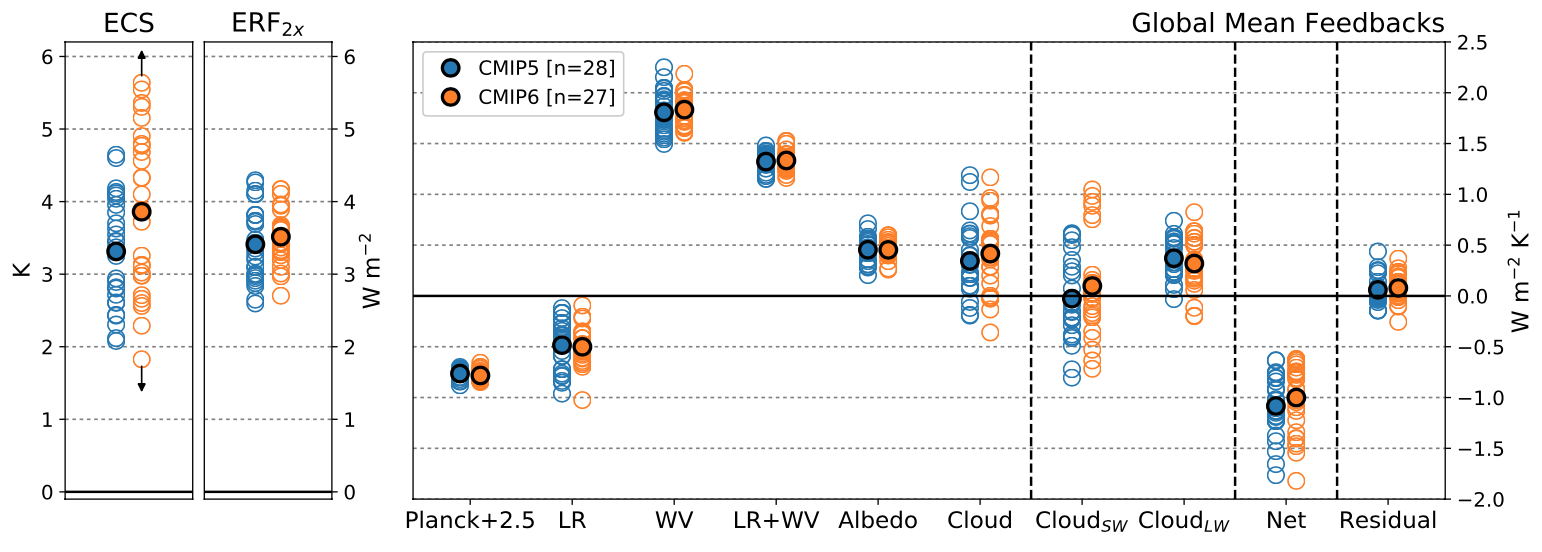
\includegraphics[width=1\linewidth]{{figs/literature_review/global_mean_cld_fbk_cmip56}.png}
	\caption{Estimates of (left) equilibrium climate sensitivity (ECS), (middle) effective radiative forcing (ERF$_{2\times}$), and (right) global mean climate feedbacks, derived from coupled experiments with abrupt quadrupling of CO$_2$ concentration experiments in CMIP5 (blue dots) and CMIP6 (orange dots) models. The black circles indicate the multi-model ensemble mean values. For display purpose, the Planck feedbacks have been added 2.5 Wm$^{-2}$K$^{-1}$ before plotting. LR and WV are lapse-rate and water vapor feedbacks, respectively. Taken from Fig. S3 of \cite{Zelinka2020causes}.}
	\label{fig:zelinka_global_mean_fbks}
\end{figure}

%\subsubsection{Water vapor feedback}
According to the Clausius--Clapeyron relation, the saturated vapor pressure is a quasi-exponential function of temperature. In addition, observations and numerical experiments consistently show that the relative humidity tends to remain more or less constant in response to climate change \citep{Held2000water,Soden2006,Goosse2010introduction}. Thus the warming will cause a significant increase in the amount of water vapor in atmosphere. Since water vapor is the dominant greenhouse gas in the atmosphere \citep{Held2000water}, the increase in water vapor content warms the atmosphere further, which in turn makes the atmosphere hold more water vapor. Thus it is a very strong positive feedback and the multi-model mean value of global mean water vapor feedback in CMIP5/6 models is about 1.8 Wm$^{-2}$K$^{-1}$ (see WV column in \figref{fig:zelinka_global_mean_fbks}).

Despite the large intermodel differences in lapse rate and water vapor feedbacks, the spread in net contribution of both feedbacks is much smaller compared to their individual spread (see LR+WV column in \figref{fig:zelinka_global_mean_fbks}). As pointed by previous studies, the lapse rate feedback and water vapor feedback are closely anti-correlated with each other \citep{Soden2006,PoChedley2018}. \cite{Soden2006} have shown that the models exhibit a nearly constant relative humidity behavior under global warming, suggesting that most of the intermodel spread in water vapor feedback does not step from the various response of relative humidity field, but from differences in the lapse rate response between models. As temperature and water vapor changes are tightly coupled in models, it is better to combine the lapse rate and water vapor feedbacks together when considering sources of intermodel spread in feedback strength \citep{Soden2006,PoChedley2018}. Another option, proposed by \cite{Held_Shell2012}, is to compute Planck and lapse rate feedbacks assuming relative rather than absolute humidity is constant, and a small feedback from changes in relative humidity quantified separately. This method can remove the cancellation between water and lapse rate feedbacks in models, so that the individual feedbacks have less scatter than in the traditional decomposition (see their Fig. 1 in \citealt{Held_Shell2012}; also see their Fig. 1 and Fig. S3 in \citealt{Zelinka2020causes}).

%\subsubsection{Surface albedo feedback}
Surface albedo feedback is related to the regions with snow and ice, which is a positive feedback that enhances climate change \citep{Winton2006surface,Goosse2018}. The mechanism is easy to understand: Warmer temperatures lead to the retreat of snow and ice, which makes the surfaces be less reflective than previous snow or ice. This causes an increase in the absorbed solar radiation and thus leads to more warming. The global mean surface albedo feedback is weak positive, and the multi-model mean value in CMIP5/6 models is about 0.5 Wm$^{-2}$K$^{-1}$ (see Albedo column in \figref{fig:zelinka_global_mean_fbks}).

% Cloud feedback
\begin{figure}[ht]
	\centering
	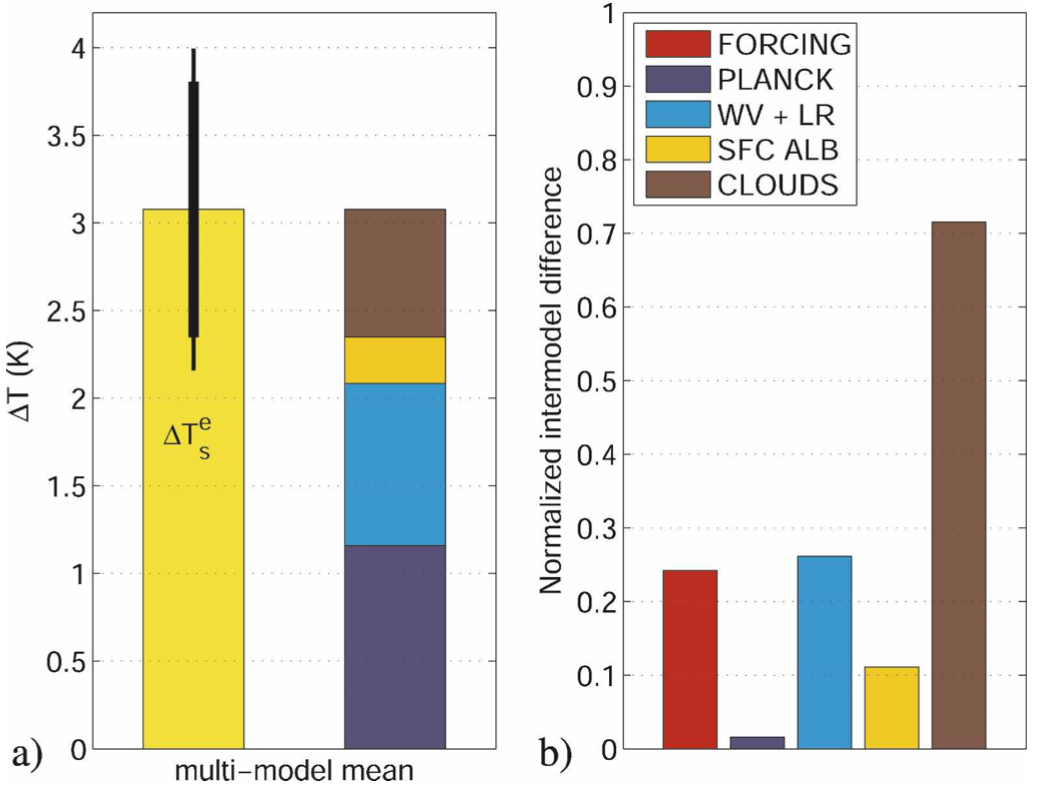
\includegraphics[width=0.8\linewidth]{{figs/literature_review/ECS_contributions}.png}
	\caption{For a CO2 doubling, (a) multi-model mean $\pm$1 standard deviation (thick line) and 5\%–95\% interval (thin line) of the equilibrium temperature change ($\Delta T^e_s$), and contributions to this temperature change associated with the Planck response, combined water vapor and lapse rate (WV+LR) feedback, surface albedo feedback, and cloud feedback. (b) Intermodel standard deviation of the temperature change estimates associated with the radiative forcing, the Planck response, and the various feedbacks normalized by the intermodel standard deviation of the equilibrium temperature change $\Delta T^e_s$ reported in (a). Taken from Fig. 1 of \cite{Dufresne2008assessment}.}
	\label{fig:ECS_contribution_from_fbks}
\end{figure}

Cloud feedback\index{cloud feedback} is the variation of cloud radiative effect at the TOA in response to global warming. In the fifth assessment report (AR5) of the Intergovernmental Panel on Climate Change (IPCC), the sign of net cloud radiative feedback is likely positive with an estimate of 0.6 Wm$^{-2}$K$^{-1}$, which, however, has a lot of uncertainties (-0.2 to 2 Wm$^{-2}$K$^{-1}$) \citep{Stocker2013}.  A recent estimate of net cloud feedback from CMIP6 models is 0.45 Wm$^{-2}$K$^{-1}$ \citep{Zelinka2020causes,Sherwood2020}, but the intermodel spread has no clear reduction from CMIP5 models (see Cloud column in \figref{fig:zelinka_global_mean_fbks}). Nevertheless, there is still no agreement on the signs of global mean net cloud feedbacks in CMIP5/6 models, and several models show the negative global mean values. Furthermore, the sign disagreements also exist in the shortwave and longwave components of cloud feedback, and are more evident in cloud shortwave components (see Cloud$_{SW}$ and Cloud$_{LW}$ columns in \figref{fig:zelinka_global_mean_fbks}). Cloud feedback is the single largest contributor to the uncertainty in the global mean net climate feedback parameters, and also contributes most to the intermodel spread of ECS \citep{Bony2005,Soden2006,Dufresne2008assessment,Colman2011tropospheric,Vial2013,Ceppi2017,Zelinka2020causes,Sherwood2020}. For instance, \figref{fig:ECS_contribution_from_fbks}, taken from \cite{Dufresne2008assessment}, quantified the contributions to ECS from different climate feedbacks, and found the cloud feedback (brown bar) is the largest source (including forcing) to the intermodel difference of ECS, although it is not the largest contributor to ECS itself. The next questions are why the intermodel spread of cloud feedback is so large, and what mechanisms control the cloud response to global warming, which are to be reviewed in next section.

%Moreover, cloud feedback is the largest uncertainty of simulated climate response to CO$_2$ foricng (i.e. climate sensitivity) in GCMs \citep{Ceppi2017,Zelinka2020causes}

%its uncertainty still the largest among all the feedback parameters (see Table 1 of \citealt{Sherwood2020}) and
%As shown in Figure \ref{fig:zelinka_global_mean_fbks}, comparing to other feedback parameters, cloud feedback has the largest intermodel spread, and is the largest uncertainty of simulated climate response to CO$_2$ foricng (i.e. climate sensitivity) in GCMs \citep{Ceppi2017,Zelinka2020causes}.

% As our understanding in cloud related processes is limited, the representation of clouds in general circulation models (GCMs) is still full of uncertainties. Moreover, the interaction between clouds and other physical parameterization schemes, and the coupling between clouds and circulation, 

\section{Clouds and cloud radiative effect}

To answer the questions proposed at the end of last section, the basic knowledge about clouds and their roles in climate system are briefly introduced first.

\begin{table}[htp]
\centering
\small %\scriptsize
\caption{Statistics of the annually averaged total cloud amount (\%) for various regions, which are from the ISCCP H-series data sets \citep{Young2018} from 1984 to 2014.}
\vspace{0.5em}
\begin{tabular}{cccc}
	\toprule
	Region & Ocean & Land &  Total\\
	\midrule
	Global & 71.7 & 54.8 & 66.1 \\
	15$^\circ$S -- 15$^\circ$N &  62.4&  63.5& 62.6 \\
	15$^\circ$N -- 35$^\circ$N &  60.1&  46.6& 55.2 \\
	15$^\circ$S -- 35$^\circ$S &  65.0&  48.3& 61.4 \\
	35$^\circ$N -- 60$^\circ$N &  80.9&  64.6& 72.5 \\
	35$^\circ$S -- 60$^\circ$S &  84.0&  65.0& 83.5 \\
	60$^\circ$N -- 90$^\circ$N &  68.9&  62.0& 66.5 \\
	60$^\circ$S -- 90$^\circ$S &  80.1&  44.3& 60.1 \\
	\bottomrule
\end{tabular}
\label{tab:statistics_cld_amt}
\end{table}

Clouds usually cover more than half areas of the Earth at any given time \citep{Houze2014,Ramanathan1989}, which is supported by recent International Satellite Cloud Climatology Project (ISCCP)\index{ISCCP} H-series products \citep{Young2018}, as shown in \tabref{tab:statistics_cld_amt}. Although they vary among different regions, the annual mean cloud amounts are usually larger than or close to 50\% at the selected regions. Also, the cloud amounts are usually larger over ocean regions than over lands, as the ocean provides a abundance of water vapor. Clouds play important roles in Earth's radiation budget and hydrological cycle, and this thesis will focus on their effect on radiation.

As shown in \figref{fig:earth_energy_budget}, clouds can exert competing influences on the energy budget of the Earth. Specifically, clouds cool the Earth by reflecting the incoming shortwave radiation emitted by the sun, and warm the planet by trapping the longwave radiation emitted by the Earth. In general, we quantify the impact of clouds on planet's radiation budget using cloud radiative effect (CRE), which is defined as the differences in TOA net radiative fluxes between all-sky and clear-sky conditions, or the upward radiative fluxes at TOA between clear-sky and all-sky conditions \citep[e.g.,][]{Ramanathan1989,Soden2004,Soden2008,Li2017}. Note that the CRE is also called cloud radiative forcing (CRF) in some literatures, but CRE is more commonly used currently, so we prefer using CRE in this study. According the definition, the shortwave and longwave CRE at TOA can be computed as follows:
\begin{equation}
    \mathrm{SWCRE} = \mathrm{SW}_{clr}^{\uparrow} - \mathrm{SW}_{all}^{\uparrow},
    \label{eq:swcre}
\end{equation}

\begin{equation}
    \mathrm{LWCRE} = \mathrm{LW}_{clr}^{\uparrow} - \mathrm{LW}_{all}^{\uparrow},
    \label{eq:lwcre}
\end{equation}
in which the subscripts $clr$ and $all$ mean clear-sky and all-sky, respectively, and the arrows indicate the direction of radiation flux. Of course, $\mathrm{SW}^{\uparrow}$ and $\mathrm{LW}^{\uparrow}$ are reflected solar radiation and OLR at the TOA, respectively. The net CRE is the sum of shortwave and longwave CREs, that is:
\begin{equation}
    \mathrm{Net~CRE} = \mathrm{SWCRE} + \mathrm{LWCRE}
    \label{eq:net_cre}
\end{equation}
The global mean shortwave CRE is approximately -50 Wm$^{-2}$, and global mean longwave CRE is around 30 Wm$^{-2}$. As the shortwave CRE dominates over the longwave CRE, the net impact of clouds on Earth's energy budget is a cooling effect with a global mean value about $-20$ Wm$^{-2}$, as shown in \figref{fig:earth_energy_budget} and \figref{fig:CRE_from_IPCC}.

The distribution of annual-mean shortwave, longwave and net CREs at TOA is displayed in \figref{fig:CRE_from_IPCC}, adapted from the Fifth Assessment Report (AR5) of the Intergovernmental Panel on Climate Change (IPCC) \citep{Stocker2013}. To better understand the spatial pattern of the CRE climatology, the CRE equations are derived in further following \cite{Ramanathan1989}. First, all-sky radiation ($R_{all}$; $R$ can be SW or LW) is rewritten as
\begin{equation}
    R_{all} = (1-C_{tot})R_{clr} + C_{tot} R_{cld} = C_{tot}(R_{cld}-R_{clr}) + R_{clr},
    \label{eq:R_all_sky}
\end{equation}
in which $C_{tot}$ is the total cloud fraction and the upward arrows in $R$ are neglected for simplicity. If we replace $R_{all}$ in \Eqref{eq:swcre} or \Eqref{eq:lwcre} with \Eqref{eq:R_all_sky}, then CRE can be expressed as follows
\begin{equation}
    \mathrm{CRE} = R_{clr}^{\uparrow} - R_{all}^{\uparrow}=C_{tot}(R_{clr}-R_{cld}).
\end{equation}

%In general, clouds can reflect the sunlight (shortwave radiation) back into space and absorb the longwave radiation emitted from the surface and cloud-free atmosphere, part of which will return to the surface. In general, the net effect of cloud is to cool the earth comparing to the cloud-free conditions. The net cooling effect of clouds is about 20 Wm$^{-2}$, which is roughly five times as large as the heating effect of doubling CO$_2$ \citep{Zelinka2017,Wild2019}. 

%Part of the reason for the large uncertainty in the future global-mean cloud radiative feedback is that clouds exert strong and competing influences on the climatological energy budget of the Earth.

%To better understand the possible mechanisms of the cloud feedback, we need to introduce the cloud radiative effect first, as clouds have competing effects on Earth's energy budget. 

\begin{figure}[ht]
	\centering
	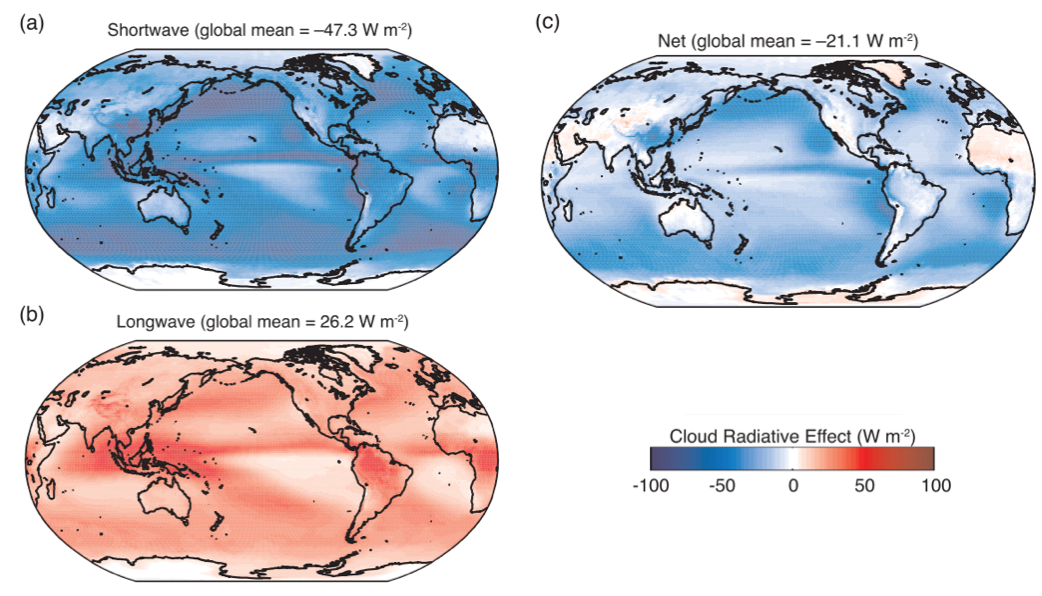
\includegraphics[width=0.9\linewidth]{{figs/literature_review/spatial_pattern_of_CRE_from_IPCC_ch7}.png}
	\caption{Distribution of annual-mean top of the atmosphere (a) shortwave, (b) longwave, (c) net cloud radiative effects averaged over the period 2001–2011 from the Clouds and the Earth’s Radiant Energy System (CERES) Energy Balanced and Filled (EBAF) Ed2.6r data set. Adapted from Fig. 7.7 of the Fifth Assessment Report (AR5) of the Intergovernmental Panel on Climate Change (IPCC) \citep{Stocker2013}.}
	\label{fig:CRE_from_IPCC}
\end{figure}

For shortwave radiation, we can write $R_{clr}=S_0\alpha_{clr}$ and $R_{cld}=S_0\alpha_{cld}$, such that shorwave CRE becomes
\begin{equation}
    \mathrm{SWCRE} = S_0 C_{tot}(\alpha_{clr}-\alpha_{cld}),
    \label{eq:swcre2}
\end{equation}
where $S_0$ is solar constant, and $\alpha_{clr}$ and $\alpha_{cld}$ are clear-sky and all-sky albedo respectively. As the clear-sky albedo usually smaller than that in all-sky (i.e. $\alpha_{clr}<\alpha_{cld}$), the shortwave CRE is negative everywhere (\figref{fig:CRE_from_IPCC}a). This means clouds reflect more sunlight back to space than clear-sky conditions, and thus the shortwave effect of clouds is to cool the Earth. In addition, the magnitude of shortwave CRE increases with cloud fraction and albedo contrast between cloudy and clear conditions, as indicated by \Eqref{eq:swcre2}.
 
\section{Cloud feedback}

\section{Cloud scheme}
\label{sec:cld_scheme_history}
\index{cloud scheme}

\subsection{Overview}
\begin{figure}[ht]
	\centering
	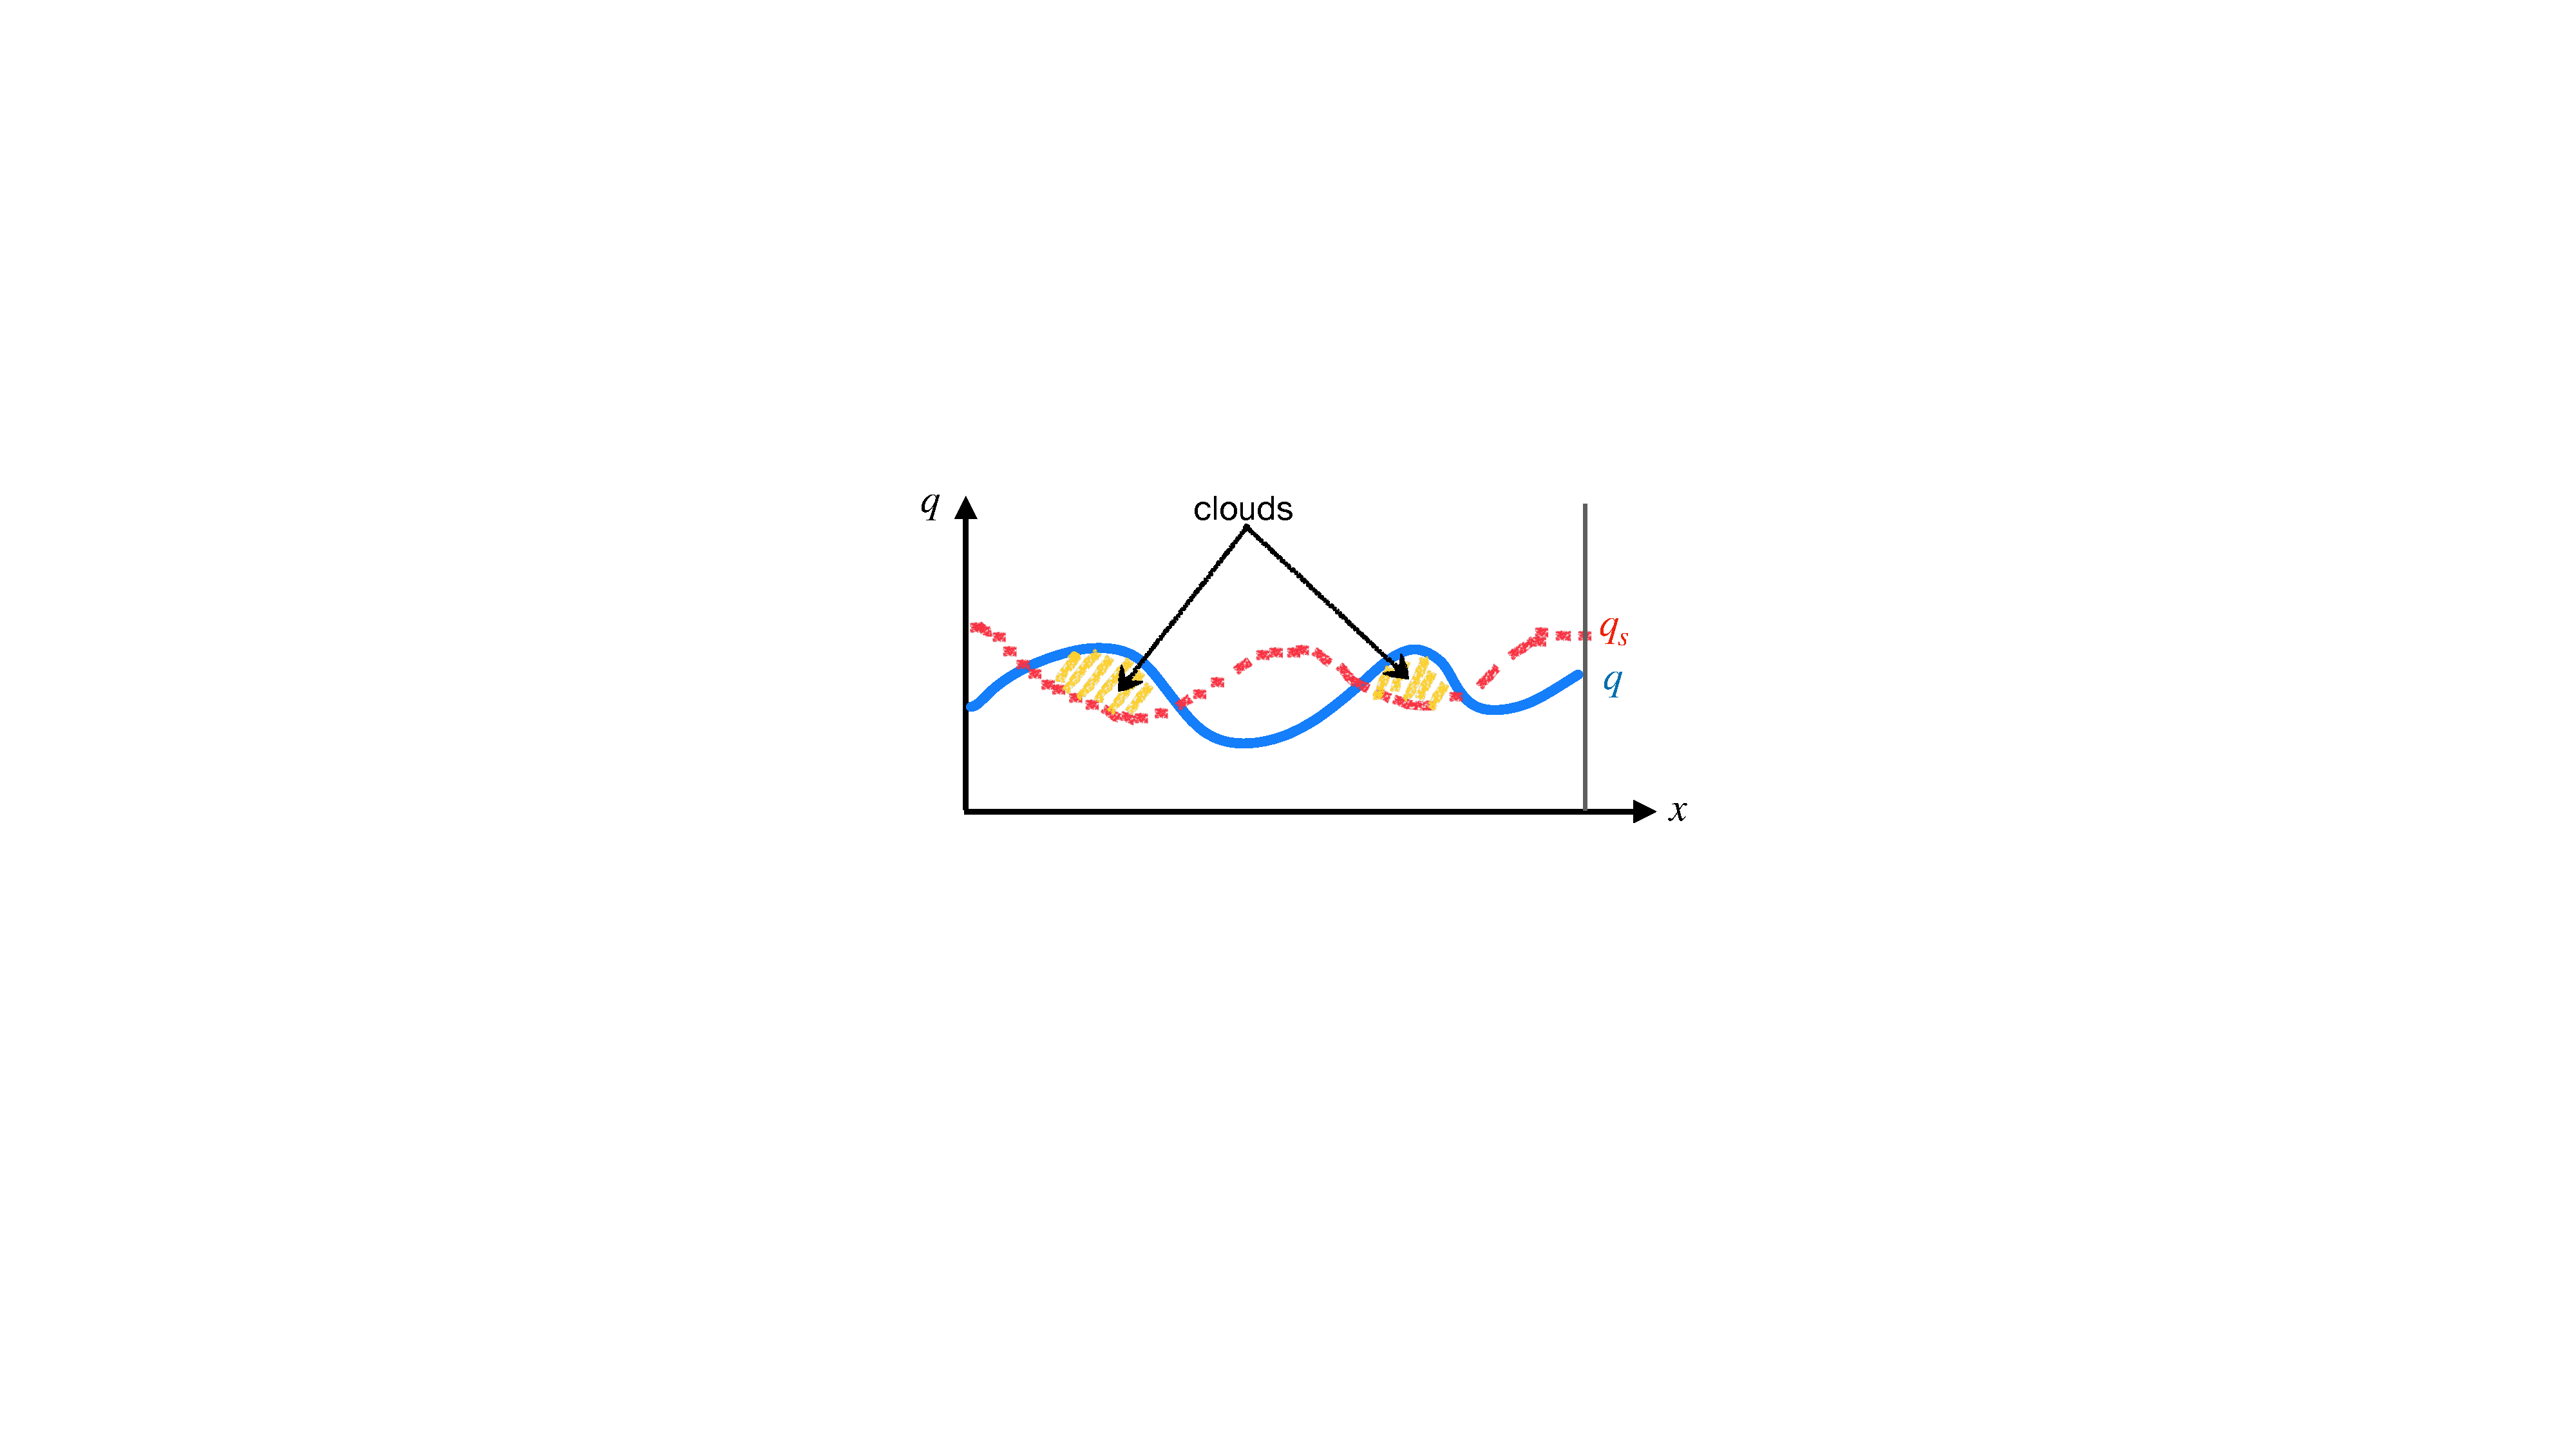
\includegraphics[width=0.8\linewidth]{{figs/literature_review/Schematic_partial_cloud_cover_in_gridbox}.pdf}
	\caption{Schematic showing that partial cloud cover in a grid box (1D) when temperature or humidity fluctuations exist. The blue line shows humidity and the red dashed line indicates saturation mixing ratio of the grid box. The shaded regions are cloudy parts as the humidity exceeds the saturation mixing ratio.}
	\label{fig:schematic_partial_clouds}
\end{figure}

At present the typical horizontal resolution of the GCMs is 50-200km, but the clouds usually involve the air motions in mesoscale and convective scale \citep{Houze2014}, which are usually in sub-grid scale both horizontally and vertically, implying that cloud processes are hard to be explicitly resolved by the GCMs. In this case, the ``parameterization" becomes a practical way to build cloud schemes. The parameterization is to represent the effects of the smaller-scale processes (turbulence, cloud microphysics, convection, etc.) in terms of the large-scale states (such as velocity, temperature, pressure, humidity) \citep{Randall2003}, which could be seen as a way to find potential relationships between the unknown and known variables \citep{Randall1989}.


\subsection{Relative humidity schemes}
\index{cloud scheme!RH scheme}
Previous studies have investigated various ways to represent clouds in climate models. For example, \cite{Holloway1971} prescribed the clouds externally with climatological data without dynamic interplay with the other components of the model. Some early modelling studies made the assumption that a grid box in the model is either fully saturated or totally unsaturated. However, this assumption is not reasonable enough as the humidity can distribute unevenly within a grid box, suggesting that condensation can occur even the relative humidity is less than 100\%. A general idea is to link the cloud cover with the relative humidity, as one can expect that the amount of condensation would increase with the increase of mean humidity of the model grid box, which is the basis for some diagnostic methods.

Diagnostic schemes predict the cloudiness based on the model variables empirically or statistically. In these schemes, the clouds can be linked to atmospheric outputs such as relative humidity, vertical velocity and static stability, among which the linear relationship between cloud fraction against RH could be simplest one. For example, \cite{Smagorinsky1960} found empirically that non-convective cloud amount correlated with the average relative humidity in the respective layers, arguing that the non-precipitating condensation depend only on the accumulated history of vertical motion, which can be reflected by the humidity. \cite{Ricketts1973} obtained roughly linear relationship between cloud amount and observed relative humidity but commented that the relationship is somewhat indefinite. %(\figref{fig:Smagorinsky_RH_cld})

Water vapor generally distributes heterogeneously in the grid box, so the averaged RH within a box should be less than 1 for a partial coverage of clouds. Previous studies usually adopt the critical relative humidity $RH_{crit}$ as the minimum threshold for clouds to form, which is often left as a free parameter that can be tuned during model development (e.g. \citealp{Hourdin2017,Kay2012,Mauritsen2012}). For example, \cite{Sundqvist1978} and \cite{Sundqvist1989} find that cloud fraction can be rewritten as a function of critical RH by assuming the water vapour is uniform distributed within the grid box. In general, $RH_{crit}$ decreases with height, but will vary according to different types of clouds. Although the $RH_{crit}$ doesn't have clear physical meaning, it can be used to modify the cloud amounts in different locations. For example, one can increase $RH_{crit}$ asymptotically to nearly unity to prevent the unrealistic circus clouds \citep{Sundqvist1989}. 

As a unique predictor, RH is very simple and useful to diagnose the cloudiness, and it is still widely used in GCMs \citep[e.g.,][]{Gordon1992,Park2014,Pope2000}. However, it is not valid for all the cases. As we can see, some studies also made use of other variables to diagnose the cloudiness. For instances, \cite{Xu1996} developed a semi-empirical scheme to determine the stratiform cloud fraction based on grid-averaged mixing ratio of condensate (cloud water and cloud ice) and RH. As for the scheme provided by \cite{Slingo1987}, both the RH and vertical velocity were taken into account, in which different empirical relations were used for different clouds including low, middle, high and convective clouds.

In summary, the methods based on relative humidity and other predictors are useful to diagnose the cloudiness, which ensures that the clouds can form before the grid box get saturated. One problem for the diagnostic methods is that in most cases the cloud condensate has to be diagnosed or prognosed via other methods \citep[e.g.,][]{Zhang2003, Park2014}, which could lead to some inconsistencies between cloud fraction and cloud condensate (e.g. \citealp{Gregory2002, Tompkins2005}).

% \begin{figure}
% 	\vspace{-0.3cm}
% 	\centering
% 	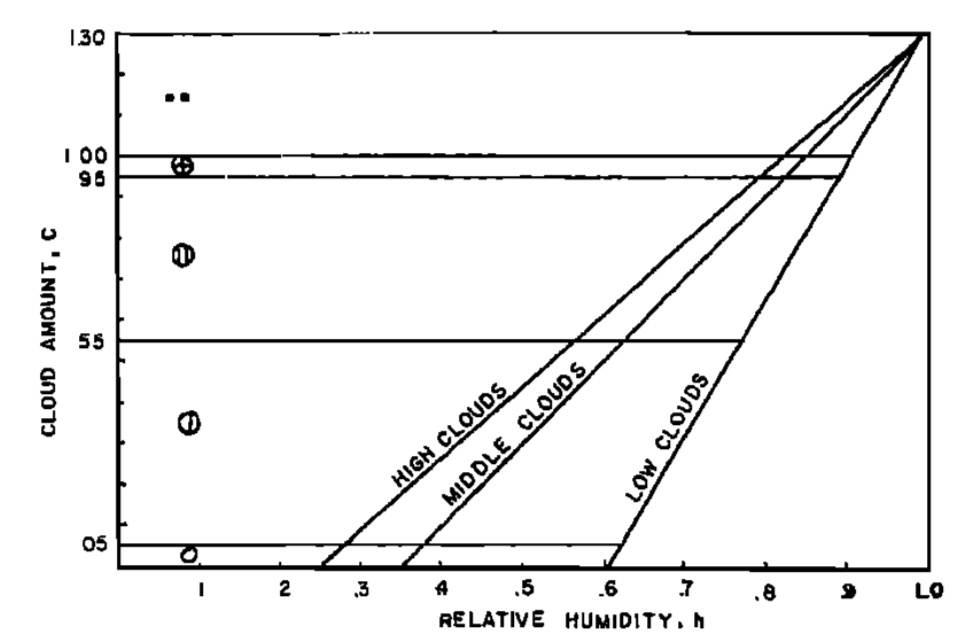
\includegraphics[width=0.6\linewidth]{{figs/literature_review/Smagorinsky1960}.png}
% 	\caption{Empirically determined relation of mean relative humidity $h$ in the layers 1000-800mb, 800-550mb and 550-300mb with cloud amount $c$ classed as low, middle and high clouds. Adapted from Figure 1 of \cite{Smagorinsky1960}.}
% 	\label{fig:Smagorinsky_RH_cld}
% \end{figure}


\subsection{Statistical schemes}
\label{sec:PDF_cld_scheme}
\index{cloud scheme!statistical or PDF scheme}

In contrast, the prognostic approach \citep[e.g.,][]{Tiedtke1993} is to explicitly calculate the clouds related variables, such as cloud water content, in order to pursuing a unification of all clouds processes, which is more realistic in some degree and requires more physical basis and interactions with other parts of the models. Another widely used cloud prediction method is statistical scheme, in which the cloud fraction and in-cloud liquid water/ice are determined based on the assumed probability distributions of subgrid variability of thermodynamic properties. As the cloud related variables such as moisture and temperature are not the same everywhere but distributed randomly within the grid box, it is natural to assume that the cloud cover depends on the distribution of moisture, sometimes on the joint distribution of moisture and temperature. As shown in a very early work, \cite{Sommeria1977} gave up the assumption that a grid is either entirely saturated or unsaturated in the climate models and proposed the idea to use the statistical distribution of moisture within the grid box. For example, given the probability distribution function (PDF) of the total water ($q_t$ is the mixing ratio) in grid box, the cloud fraction ($CF$) can be calculated as 
\begin{equation}
    CF=\int_{q_s}^{\infty}\text{PDF}(q_t)\operatorname{d}q_t,
\end{equation}
and the cloud water content ($q_c$ is the mixing ratio of cloud water) is
\begin{equation}
    q_c=\int_{q_s}^{\infty}(q_t-q_s)\text{PDF}(q_t)\operatorname{d}q_t,
\end{equation}
where $q_s$ is the saturation mixing ratio in both formulations.

However, the shapes of subgrid-scale PDF of total water specific humidity, saturation deficit, or a combined variable of liquid water and potential temperature are difficult to determine due to limit of observational data, so sometimes the model data are also used \citep{Bony2001}. Additionally, many different PDF forms have been proposed in the previous studies. For example, \cite{LeTreut1991} made use of the uniform distribution of total water in the grid box to calculate the clouds cover and liquid water content. Other symmetrical distributions, such as Gaussian distribution \citep{Sommeria1977}, triangular distribution \citep{Smith1990} and skewed distributions, such as lognormal distribution \citep{Bony2001} and beta distribution \citep{Tompkins2002}, have also been employed in numerical models. However, there are also some problems in the distributions. For example, the Gaussian distribution is unbounded, indicating that the maximum cloud condensate mixing ratio might approach infinity, and cloud cover is always large than zero \citep{Tompkins2002}. In general, complicated forms of the PDF need more parameters to fit. But due to the limitation of the data, it is possibly hard to validate the distributions. Linking the statistical cloud scheme to other physical processes seems a promising way to improve cloud simulations. For example, \cite{Qin2018} developed a Gaussian PDF cloud scheme with the PDF variance diagnosed from the turbulent
and shallow convective processes, which could improve the simulation of low marine clouds and alleviate double Intertropical Convergence Zone (ITCZ) problem \citep{Qin2018alleviated}.

The statistical cloud schemes may have better performance than the diagnostic ones, but considering the fact that there is no clouds scheme in Isca currently, it would be useful to implement the simple diagnostic schemes in Isca first, which can be seen as the first step to implemented a hierarchy of cloud schemes.

\subsection{Relationship between relative humidity and statistical schemes}

As discussed in previous section, one has to determine the expression of sub-grid variance (i.e. second order moment) or other higher-order moments in the statistical schemes. In doing so there are two general practices in current studies. The simple case is to use the time-invariant variance \citep[e.g.,][]{Sundqvist1978,Smith1990}, and the other approach is to employ time varying variance, which are usually obtained from other physical processes such as boundary layer scheme or shallow convection schemes \citep[e.g.,][]{Qin2018}. The second case usually provides a more realistic link between clouds and other physical processes \citep{Tompkins2002}. 

Note that there is no distinction between the RH schemes and statistical schemes, although they seem different in forms. As a matter of fact, if the subgrid variance in a statistical scheme is assumed to be time-invariant, it can be reduced to a RH scheme \citep{Tompkins2002,Tompkins2005}. The key is to link the variance with the critical relative humidity. That is to say, critical RH value can reflect the level of sub-grid variance in RH schemes \citep{Quaas2012}. Larger critical RH value means the lower subgrid variability and vice versa. For example, the \cite{Sundqvist1978} RH scheme can be derived by assuming a uniform distribution of total water mixing ratio within a grid box, in which the variance is assumed a constant fraction of the saturation water vapor mixing ratio, and this constant is associated with critical RH value (see Appendix A of \cite{Quaas2012} for a full derivation). Another example is the triangular distribution used by \cite{Smith1990} and \cite{Park2014}, they also obtain the equivalent RH formulation by assuming the variance is related to critical RH. As pointed by \cite{Tompkins2002}, the parameterizations such as \cite{Xu1996}, in which cloud fraction is related to RH and cloud condensate, can be viewed as manifestations of a statistical scheme although where the actual PDF of total water is not known. %, but the time-mean statistics of its integral are.

\section{Research questions and thesis outline}
\label{sec:thesis_layout}

The thesis is arranged as follows:

\chapref{ch:introduction} introduces the backgrounds, motivation, aims and outline of this study. The background parts include the basic ideas of Earth's radiation budget, climate feedback and cloud radiative effect and its feedback.

\chapref{ch:methods} describes the data and methods used in the thesis. The data sets include the satellite observations about clouds and radiation, and other climate variables, such as temperature, relative humidity and vertical velocity, from the reanalysis. The methodology part first gives a brief introduction of Isca model, then presents the methods used in the thesis to calculate climate feedback. This should have two parts: First is about how to employ kernel method in Isca to estimate Planck, lapse rate, water vapor feedbacks for gray and RRTM radiation schemes; Second is to compare the methods to calculate the cloud feedback. Finally, several low cloud proxies used in \chapref{ch:simple_cld_scheme} is listed for reference.

\chapref{ch:polaramplification} mainly presents the results from polar amplification of temperature change in varying albedo simulations. In this chapter, the contributions from different climate feedbacks, forcing and heat transport are quantified through the decomposition method. The major conclusion is that the local lapse rate feedback and Planck feedback (plus heat transport) play important role in determining the warming structure in polar region.

\chapref{ch:simple_cld_scheme} focuses on the parameterization of simple cloud scheme and the evaluation of its simulation of cloud climatology. These include the parameterization of the cloud fraction and cloud optical properties, simulation setup and the comparison of the simulated cloud fraction, radiative flux and cloud radiative effect with observations and CMIP5 models. The comparison consists of the spatial pattern, zonal mean structure and seasonal cycle. %Basically, this chapter is modified from the GMD manuscript. The content to be added is the sensitivity of the scheme to horizontal and vertical resolutions.

The topic of \chapref{ch:cld_fbk} is cloud feedback. First, the cloud feedback simulated from the simple cloud scheme is evaluated. The spatial patterns of longwave, shortwave and net cloud feedbacks, as well as their components such as cloud amount, altitude and optical depth feedbacks, will be investigated and compared with the CMIP models. The possible reasons for the feedback features are to be explored. Then the results from perturbed parameter ensemble (PPE) will be analysed. The cloud feedback spread from the PPE will be checked to see if they could `reproduce' such spread in CMIP models. The causes to the cloud feedback spread in the PPE will be investigated. Base on these results, which parameter or process is more sensitive would be analysed. Finally, the implications for equilibrium climate sensitivity will be discussed.

\chapref{ch:conclusion} summarises the major contents and conclusions of the thesis, and discusses the possible future work.
